% Block diagram of the CPU, rendered to cpu.png by "make diagrams" (see the
% BLOCK_DIAGRAMS variable in the top-level Makefile).
%
% This replaces an earlier cpu.drawio / cpu.png pair, which had no reproducible
% source: it was built in the diagrams.net GUI and could only be edited there.
% Anything that changes the module hierarchy has to change this file too, so
% keeping the source as text next to the RTL is the point.
%
% What it shows, and what it deliberately does not: the six blocks of the
% pipeline in pipeline order, the two shared modules they hang off (REGISTERS
% on the left, MEMORY on the right), the two Wishbone buses leaving on the
% right, and the dotted boundary of CPU_MAIN. It does NOT show the valid/ready
% handshaking, the redirect paths from WRITE and DECODE back to FETCH, or the
% bank-switch signals -- those are described in doc/README.md and in the
% per-module READMEs, and drawing them here would turn the picture into a net
% list.
%
% The short black bars are the pipeline registers that set the loop's latency:
% every clock cycle a beat spends going round is one of them. There are seven,
% and where they are NOT is as informative as where they are.
%
%   FETCH, at the base of the instruction-address arrow  wb_addr_o (p_wishbone)
%   the instruction memory, at the far end of that arrow dp_ram's read register
%   ICACHE, at its output                                m_data_o
%   DECODE, at its output                                seq_stage_o (p_output)
%   REGISTERS, in the middle                             dp_ram's read register
%   PREPARE, at its output                               wr_stage_o (p_output)
%   the data memory, at the far end of its address arrow dp_ram's read register
%
% SEQUENCER, WRITE and MEMORY have none. SEQUENCER's p_output is a
% "process (all)" that slices one microcode chunk out of DECODE's registered
% list; WRITE's p_reg is likewise combinational, which is why reg_addr_o,
% fetch_addr_o and fetch_valid_o are decoded within the cycle and are the
% design's timing-critical nets; and MEMORY buffers its Wishbone request in a
% one_stage_buffer and its responses in one_stage_buffers, all of which cut
% through combinationally when empty. So on both the instruction and the data
% side the register that ends the round trip belongs to the RAM, not to the
% module in front of it -- hence the two bars sitting on the bus arrows rather
% than inside a block. doc/loop_timing.tex draws the same fact as a waveform.

\documentclass[border=8pt]{standalone}

\usepackage[T1]{fontenc}
\usepackage{helvet}
\renewcommand{\familydefault}{\sfdefault}

\usepackage{tikz}
\usetikzlibrary{arrows.meta, positioning, shapes.arrows, fit, calc}

\begin{document}

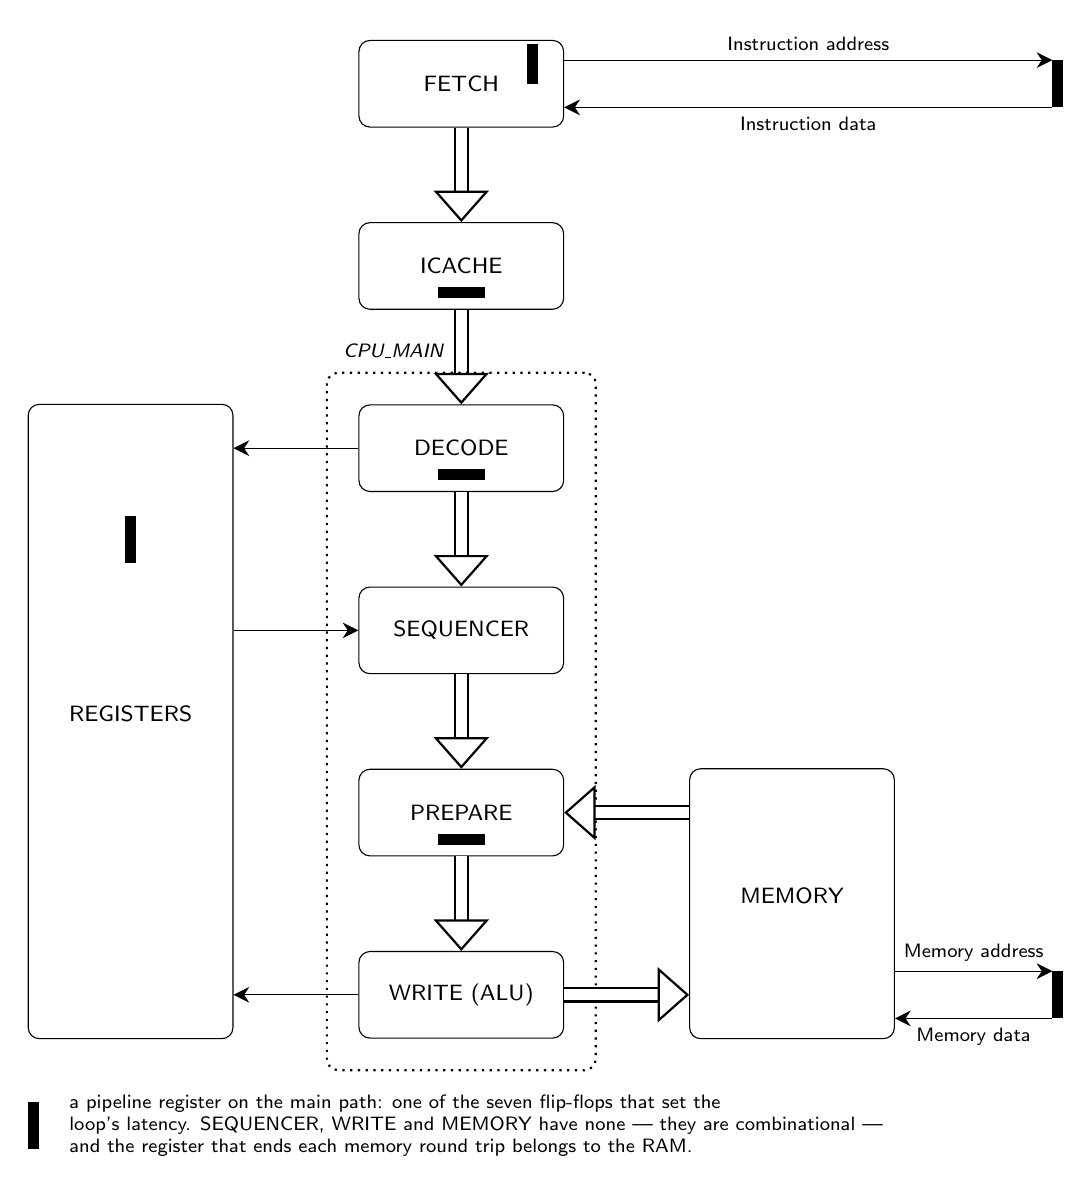
\begin{tikzpicture}[
      font = \sffamily\footnotesize,
      % A pipeline stage, or one of the two shared modules.
      block/.style = {
         draw,
         rounded corners = 4pt,
         minimum width   = 26mm,
         minimum height  = 11mm,
         align           = center
      },
      % The fat hollow arrows of the original diagram: the pipeline's data
      % path, one instruction (or micro-operation) per beat. A doubled line
      % with an open tip draws the same outlined block arrow that the
      % diagrams.net original used.
      %
      % The line width is pinned, and must stay at or above ~0.5pt. "double"
      % strokes the path once in black at (2*line width + double distance) and
      % then again in white at (double distance), leaving the two visible lines
      % as slivers exactly one line width thick. At the default 0.4pt that is
      % 0.83px at the 150dpi "make diagrams" renders at -- thinner than a pixel,
      % so whether a sliver survives rasterisation depends on where it happens
      % to fall on the pixel grid. It cost the lower line of the WRITE-to-MEMORY
      % arrow, which was correct in the PDF and simply absent from the PNG.
      flow/.style = {
         draw,
         thick,
         double,
         double distance = 4pt,
         -{Triangle[open, length = 4mm, width = 7mm]}
      },
      % Thin arrows: everything that is not the pipeline data path.
      wire/.style   = {draw, -{Stealth[length=2mm, width=2mm]}},
      % "above" or "below" is chosen per arrow, so that the two labels of a
      % bus pair sit outside the pair rather than in the gap between them.
      buslabel/.style = {midway, font = \sffamily\scriptsize},
      % A pipeline register, drawn as a short bar ACROSS the path it cuts, so
      % that the bar's long axis is always perpendicular to the flow: ffh for
      % the vertical pipeline arrows, ffv for the horizontal buses. Both are
      % 6mm long, which is exactly the 3mm-either-side spacing of a bus pair,
      % so a bar dropped between the two arrows of a pair touches both.
      ffh/.style = {fill = black, inner sep = 0pt,
                    minimum width = 6mm, minimum height = 1.4mm},
      ffv/.style = {fill = black, inner sep = 0pt,
                    minimum width = 1.4mm, minimum height = 6mm}
   ]

   %% ---------------------------------------------------------------
   %% The pipeline, top to bottom
   %% ---------------------------------------------------------------

   \node[block]                            (fetch)   {FETCH};
   \node[block, below = 12mm of fetch]     (icache)  {ICACHE};
   \node[block, below = 12mm of icache]    (decode)  {DECODE};
   \node[block, below = 12mm of decode]    (seq)     {SEQUENCER};
   \node[block, below = 12mm of seq]       (prepare) {PREPARE};
   \node[block, below = 12mm of prepare]   (write)   {WRITE (ALU)};

   \draw[flow] (fetch)   -- (icache);
   \draw[flow] (icache)  -- (decode);
   \draw[flow] (decode)  -- (seq);
   \draw[flow] (seq)     -- (prepare);
   \draw[flow] (prepare) -- (write);

   %% ---------------------------------------------------------------
   %% CPU_MAIN
   %% ---------------------------------------------------------------

   % The label rides just above the top edge rather than inside it: the
   % ICACHE-to-DECODE arrow comes down the centre line, and CPU_MAIN set inside
   % the box is wide enough to run into its shaft.
   \node[draw, dotted, thick, rounded corners = 4pt, inner sep = 4mm,
         fit = (decode) (seq) (prepare) (write)] (cpumain) {};
   \node[anchor = south west, font = \sffamily\scriptsize\itshape]
      at ([xshift = 1mm, yshift = 0.5mm] cpumain.north west) {CPU\_MAIN};

   %% ---------------------------------------------------------------
   %% Shared modules: REGISTERS on the left, MEMORY on the right
   %% ---------------------------------------------------------------

   % Both boxes are fitted to a full-width RECTANGLE -- the two corners are
   % offset by half of block's 26mm minimum width -- rather than to the
   % zero-width vertical segment (regx |- ...) (regx |- ...) that would
   % otherwise say the same thing. The shape comes out identical either way,
   % because minimum width expands it, but the LABEL does not: fitted to a
   % zero-width box it ends up 6mm right of centre, all but touching the right
   % border. Keep the two x-offsets 26mm apart and centred on regx/memx.

   % REGISTERS spans DECODE down to WRITE: DECODE issues the reads, the values
   % come back into SEQUENCER, and WRITE writes.
   \coordinate (regx) at ([xshift = -42mm] decode.center);
   \node[block, inner sep = 0pt,
         fit = {([xshift = -13mm] regx |- decode.north)
                ([xshift =  13mm] regx |- write.south)}] (regs) {REGISTERS};

   % MEMORY spans PREPARE down to WRITE: WRITE issues the requests, PREPARE
   % consumes the read responses.
   \coordinate (memx) at ([xshift = 42mm] decode.center);
   \node[block, inner sep = 0pt,
         fit = {([xshift = -13mm] memx |- prepare.north)
                ([xshift =  13mm] memx |- write.south)}] (memory) {MEMORY};

   %% ---------------------------------------------------------------
   %% Connections
   %% ---------------------------------------------------------------

   % Operand reads: the register numbers leave DECODE, and the values come back
   % a clock cycle later -- by which time the instruction has moved on, so they
   % are wired to SEQUENCER rather than back into DECODE.
   \draw[wire] (decode.west) -- (regs.east |- decode.west);
   \draw[wire] (regs.east |- seq.west) -- (seq.west);
   % Result write-back, plus the pre/post-increment write-backs.
   \draw[wire] (write.west) -- (regs.east |- write.west);

   % Read responses back into PREPARE, requests out of WRITE.
   \draw[flow] (memory.west |- prepare.east) -- (prepare.east);
   \draw[flow] (write.east) -- (memory.west |- write.east);

   %% ---------------------------------------------------------------
   %% The two Wishbone buses
   %% ---------------------------------------------------------------

   % Each bus is drawn as the pair it is: the address leaves the CPU, the data
   % comes back. The two arrows of a pair are 3mm either side of the edge
   % anchor they would otherwise share, which keeps both inside the 11mm height
   % of the box they attach to.
   \coordinate (busx)  at ([xshift = 20mm] memory.east);
   \coordinate (ibusl) at (fetch.east);
   \coordinate (ibusr) at (busx |- fetch.east);
   \coordinate (dbusl) at (memory.east |- write.east);
   \coordinate (dbusr) at (busx |- write.east);

   \draw[wire] ([yshift =  3mm] ibusl) -- ([yshift =  3mm] ibusr)
      node[buslabel, above] {Instruction address};
   \draw[wire] ([yshift = -3mm] ibusr) -- ([yshift = -3mm] ibusl)
      node[buslabel, below] {Instruction data};

   \draw[wire] ([yshift =  3mm] dbusl) -- ([yshift =  3mm] dbusr)
      node[buslabel, above] {Memory address};
   \draw[wire] ([yshift = -3mm] dbusr) -- ([yshift = -3mm] dbusl)
      node[buslabel, below] {Memory data};

   %% ---------------------------------------------------------------
   %% The pipeline registers
   %% ---------------------------------------------------------------
   %
   % Drawn last, so that a bar sits on top of the arrow it cuts rather than
   % under it. See the header for which register each one is.

   % FETCH/wb_addr_o, at the base of the instruction-address arrow. This is the
   % one bar that is not 6mm long: the arrow leaves 3mm above centre and the
   % block is only 11mm tall, so a full-length bar centred on the arrow would
   % poke out through the top edge.
   \node[ffv, minimum height = 5mm] at ([xshift = -4mm, yshift = 2.5mm] fetch.east) {};

   % ICACHE/m_data_o, DECODE/seq_stage_o, PREPARE/wr_stage_o: each at the
   % bottom of its own block, cutting the outgoing pipeline arrow. Note the
   % three blocks BETWEEN them -- SEQUENCER, and WRITE, and (on the right)
   % MEMORY -- get nothing, which is the point of the whole annotation.
   \node[ffh] at ([yshift = 2.2mm] icache.south)  {};
   \node[ffh] at ([yshift = 2.2mm] decode.south)  {};
   \node[ffh] at ([yshift = 2.2mm] prepare.south) {};

   % REGISTERS' dp_ram read register, in the middle of the block: DECODE
   % presents the register numbers on the upper wire and the values come back
   % on the lower one a clock cycle later, which is exactly this flip-flop.
   % Placed halfway between those two wires, so it is well clear of the label.
   \coordinate (regff) at ($ (decode.west)!0.5!(seq.west) $);
   \node[ffv] at (regff -| regs.center) {};

   % The two RAM read registers. Each sits at the far end of an address arrow,
   % just outside the CPU, and is 6mm long -- exactly the 3mm-either-side
   % spacing of a bus pair -- so it touches the address arrow that ends on it
   % and the data arrow that starts from it.
   \node[ffv] at ([xshift = 0.7mm] ibusr) {};
   \node[ffv] at ([xshift = 0.7mm] dbusr) {};

   %% ---------------------------------------------------------------
   %% Legend
   %% ---------------------------------------------------------------

   % Below REGISTERS, in the empty band under the diagram. It has to clear the
   % bottom edge of the CPU_MAIN box, which is 4mm below write.south.
   \node[ffv, anchor = west] (legendff) at ([yshift = -11mm] regs.south west) {};
   \node[anchor = west, font = \sffamily\scriptsize, align = left]
      at ([xshift = 2.5mm] legendff.east)
      {a pipeline register on the main path: one of the seven flip-flops that set the\\
       loop's latency. SEQUENCER, WRITE and MEMORY have none --- they are combinational ---\\
       and the register that ends each memory round trip belongs to the RAM.};

\end{tikzpicture}

\end{document}
